\documentclass[11pt, a4paper]{article}
\usepackage[utf8x]{inputenc}
\usepackage[swedish, english]{babel}		% last is active
\usepackage{graphicx}
\usepackage{amsmath}					% to be able to \split eqs
\usepackage{amssymb}					% Real/Imaginary fonts
\usepackage{units}
\usepackage[tight, hang]{subfigure}
\usepackage{url}
\usepackage{tikz}						% for drawing
\usetikzlibrary{shapes, arrows, decorations.markings, decorations.pathmorphing, decorations.pathreplacing, calc}
\usepackage{fancyhdr}
\usepackage{float}						% H-positioned and custom floats
\usepackage{datetime}					% to fix date format
\usepackage[usenames,dvipsnames]{pstricks}
%\usepackage{epsfig}
%\usepackage{pst-grad} % For gradients
%\usepackage{pst-plot} % For axes
\usepackage{pgfplots}
% =================== some local stuff ================= %
\newcommand{\degree}{\ensuremath{^\circ}}
\newcommand{\todayswe}{\the\year-\twodigit\month-\twodigit\day}


\def\contacts{Torbjørn Ludvigsen, tolu0022@student.umu.se\\Olof Lenti, olle0004@student.umu.se\\
Yunus Gures, yunusgures@gmail.com}
\def\names{Torbjørn Ludvigsen, Olof Lenti, Yunus Gures}
\def\dept{Department of Physics}
\def\course{Non-invasive measurement techniques}
\def\lab{Optical measurements:\\Determination of the Damping of a Pendulum with Time of Flight}
\def\supervisors{Patrick Ehlers\\Isak Silander\\ Amir Khodabakhsh}
\date{\todayswe}
% custom commands
\newcommand\OpVec[1]{\boldsymbol{\hat{#1}}}		% bold with hat for operator vectors
%\newcommand\Sup[1]{\textsuperscript{\tiny{#1}}}		% 1st, 2nd.. and so on
\newenvironment{eqn}{\begin{equation*} \begin{split}}{\end{equation*} \end{split}}
% header

% document
\begin{document}
\pagestyle{fancy}
\begin{titlepage}
	\begin{center}
		\course\\
		\Large{\lab}\vspace{2mm}
		\hrule\vspace{2mm}
		\tiny{\contacts}\vspace{2mm}
		\hrule
	\end{center}
	\vspace{4mm}

	\begin{abstract}

  $\alpha_{alu} =\unit[(23.0 \pm 0.1)\cdot10^{-6}]{K^{-1}}$ 

  $\alpha_{sst} = \unit[(15.8 \pm 0.2)\cdot10^{-6}]{K^{-1}}$, 
    which is only 1 \% off tabulated values \cite{ph, thex}.

	\end{abstract}
	\vfill
	\hrule\vspace{2mm}
	\centering
		\tiny{Supervisor: \supervisors}
	%\end{center}
\end{titlepage}

\pagestyle{plain}
\vspace{2cm}
\section{Introduction}
A mechanical system cosisting only of a rigid body, with only one degree of 
freedom, rotation around a constant axis, from here on called a pendulum, is 
a system of great interest. Historically it has had a wide range of
applications in science, mathemathics and in everyday life. Among the reasons for
its continued importance as an educational tool in physics is its short, general 
equations of
motion in the linearized, small amplitude case, and the ease and the great number 
of ways by which this case can be extended.

This experiment in particular will measure a physical pendulum's decreasing velocity
in order to find and analyze its damping forces. A time of flight instrumentation
is constructed and used to aquire the velocity data.

\section{Theory}
\subsection{The pendulum}
For a simple rigid body pendulum, Newtons second law gives us the following
equation of motion:
\begin{equation}
  I_p\frac{\d^2\theta}{\dt^2} + mgl\sin{\theta} = 0
  \label{eq_of_motion}
\end{equation}



\subsection{Friction}

\subsection{Damping}

\subsection{Optics}
\subsection{Circuits}
\subsection{maths}

The forces considering air drag are described differently for different velocities. For very low velocities i.e. when the pendulum is at its turning point the drag force will be proportional to the velocity as

\[
F_d = -bv,
\]
where $F_d$ is force of drag, $v$ is the velocity and $b$ is a positive constant.
For higher velocities the force of 





By beginning with the equation
\[
v_{max} = Ce^{at} + De^{bt}.
\]
By breaking out $e^{at}$ and taking the logarithm we end up with the equation
\[
\ln(v_{max}) = \ln(C + De^{\frac{b}{a}t}) + at
\]
For small $t$ the first term will be nearly constant. A linear fit can be made to find the slope $a$.
In a similar fashion we can break out $e^{bt}$

\section{Experimental Setup}
\section{Procedure}

\section{Error calculations}
\subsection{Error of the time of flight instrumentation}
One error of the measurement device is the error from the non-continous data collecting as demonstrated in Figure \ref{f:lasercloseup}.
Since our LabVIEW-setup collect data only at a rate of some $kHz$ and we measure fast velocities we will get an error from this. The error can be found as
\[
	v_{err}=\Delta t_{err}\cdot \Delta s,
\]
where $\Delta s$ is the length between the two laser lights, $\Delta t$ is the rate of the data collecting and $v$ is the velocity. The error in time is $<\Delta t$. Thus we set the maximum error in time as $\Delta t$.
\begin{figure}[h]
	\centering
	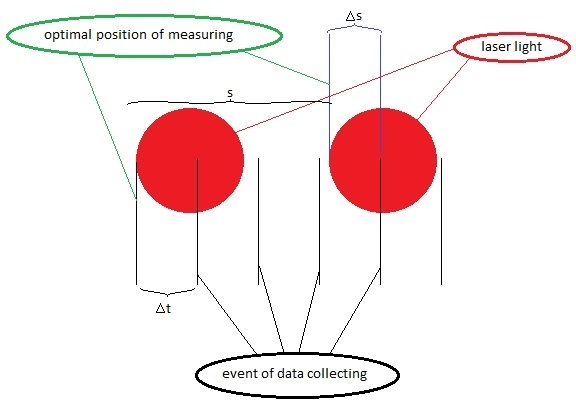
\includegraphics{errorofdevice}
	\caption{The source of the error of the time of flight instrumentation is demonstrated.}
	\label{f:lasercloseup}
\end{figure}
By the fact that $\Delta s = v\cdot (\Delta t + \Delta t_{err})$We set $\Delta t = 50kHz$.


\subsection{Error of the slope of a linear fitting}
To calculate the error of the slope of a linear fit we simply use MATLAB to calculate the following equation:
\begin{equation}
	s = \text{std}(f(x)-data(x)),
	\label{e:std}
\end{equation}
where $s$ is the standard deviation of the residuals, $x$ is the x-values of the region considered, $data$ is the data values of the region considered and $f$ is the linear fit.
This standard deviation will be a measure of how correct the linear approximation is.



\section{Results}
In Figure \ref{f:nopaper} we see the logarithm of work done by the friction and 
drag on the pendulum with the added area plotted versus the logarithm of velocity. 
The units of the work and velocity are an unknown constant times their SI-unit. 
The slopes and the errors of the linear fits of the two different regions of the plot are calculated to be
\[
	slope_{low}=\frac{\Delta\ln(W_{low})}{\Delta\ln(v_{low})} = 1.36(4),
\]\[
	slope_{high}=\frac{\Delta\ln(W_{high})}{\Delta\ln(v_{high})} = 2.60(3).
\]
The values inside the parentheses are the standard deviation of the slope calculated using Equation \ref{e:std}.

\begin{figure}[h]
	\centering
	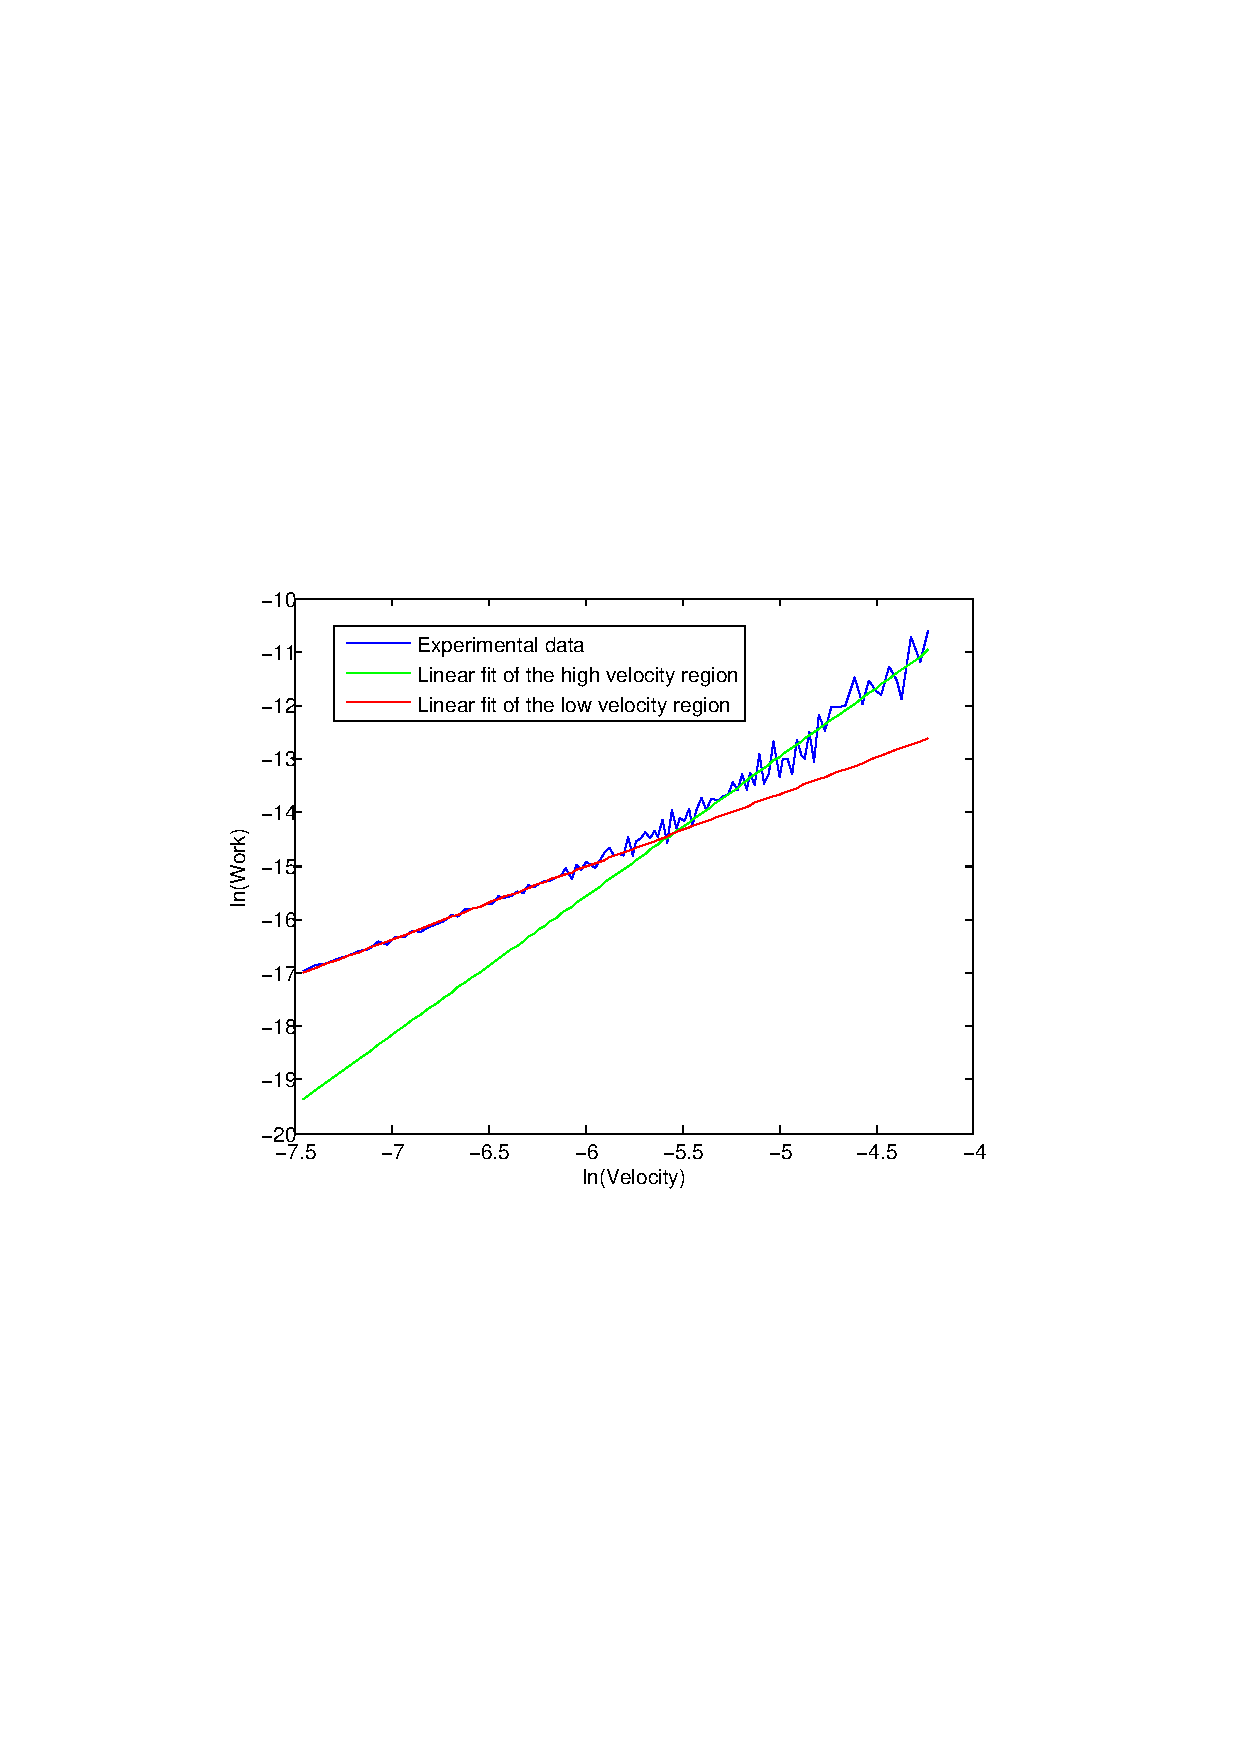
\includegraphics[trim=10.0cm 10.0cm 10.0cm 10.0cm, scale=0.7]{no_paper}
	\caption{Work versus velocity data and  linear fits for the pendulum.}
	\label{f:nopaper}
\end{figure}

In Figure \ref{f:paper} we see the logarithm of work done by the friction and 
drag on the pendulum with the added area plotted versus the logarithm of velocity. 
The units of the work and velocity are an unknown constant times their SI-unit. 
The slopes and the errors of the linear fits of the two different regions of the plot are calculated to be

\[
	slope_{low}=\frac{\Delta\ln(W_{low})}{\Delta\ln(v_{low})} = 1.96(4),
\]\[
	slope_{high}=\frac{\Delta\ln(W_{high})}{\Delta\ln(v_{high})} = 2.63(7).
\]

\begin{figure}[h]
	\centering
	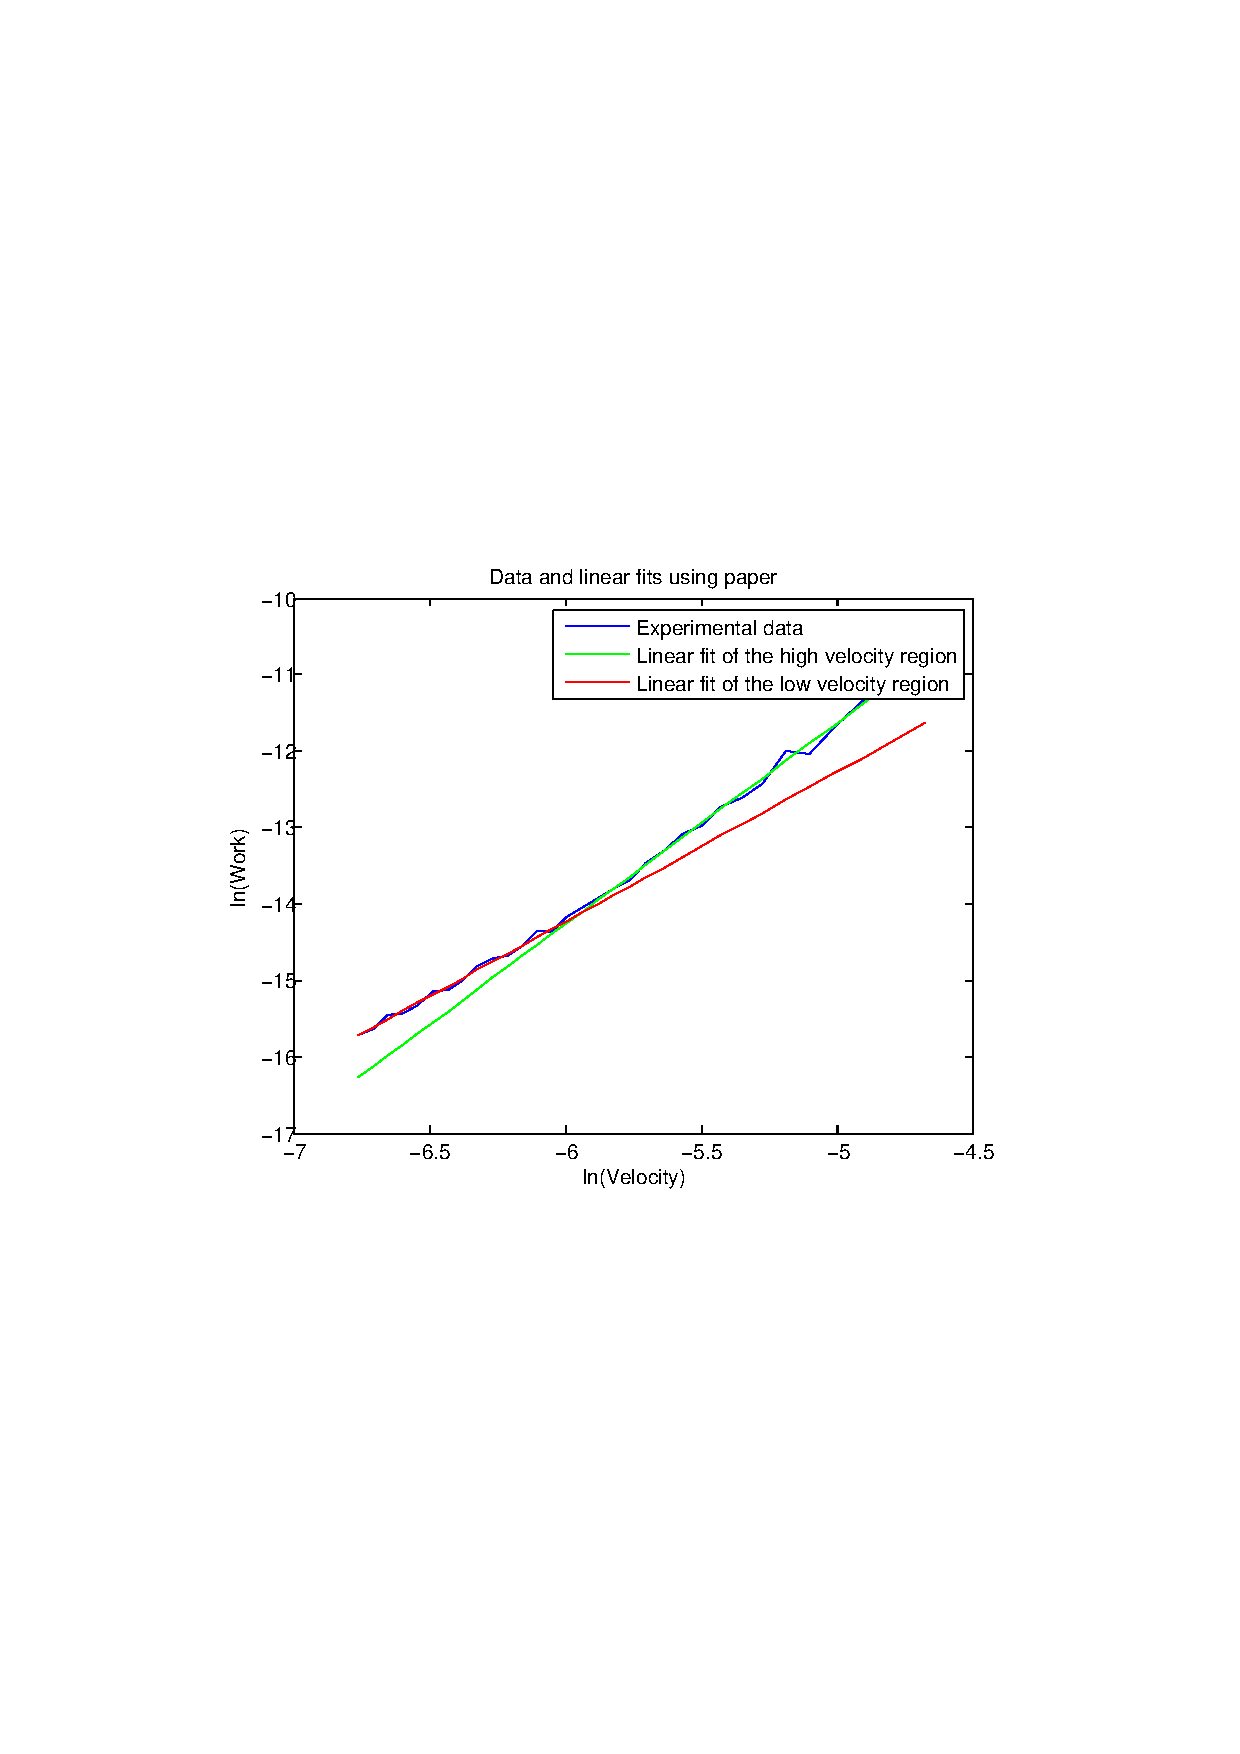
\includegraphics[trim=10.0cm 10.0cm 10.0cm 10.0cm, scale=0.7]{paper}
	\caption{Work versus velocity data and  linear fits for the pendulum with an added area.}
	\label{f:paper}
\end{figure}

It is clear that the slopes of the high velocity region are similar and close to $3$. 
The slope of the added-area pendulum for the low-velocity region is very close to $2$.
The slope of the ordinary pendulum for the low-velocity region is slightly above $1$.



\section{Discussion}
The behavior of the high-velocity region is not entirely as expected. We expected the slope of the added-area pendulum 
to be closer to $3$ than the other pendulum.
This is explained by the fact that the high-velocity regions are not exactly the same for the different types of pendula. We were not 
able to do a high enough velocity measurement due to the quick damping as well as the fluttering of the added area.
\section{Summary and Conclusions}
\vfill

\begin{thebibliography}{99}
	\bibitem{ph} Nordling, C., Österman, J. (2006). 
  \textit{Physics Handbook  $8^{th}$}\\
  Lund, Sweden, Studentlitteratur.

  \bibitem{drag} Wikipedia. \textit{Drag}\\ 
  \url{http://en.wikipedia.org/wiki/Drag_(physics)} [\todayswe]

\end{thebibliography}

\begin{appendix}
\end{appendix}

% nY KOMMENTAR

\end{document}
%\begin{figure}[H]
%	\centering
%	\begin{tikzpicture}[scale = 0.95]
%		\def\mr{1.5};
%		\draw (0,0) ellipse (0.5 and \mr);
%		\begin{scope}
%			\clip (0,0) ellipse (0.5 and \mr);
%			\foreach \i in {0, 1, ..., 15} {
%				\draw (-0.5, {-3 + 0.25*\i}) -- (0.5, {-1 + 0.25 * \i});
%			}
%		\end{scope}
%		\path[fill = white, opacity = 0.7] (0, 0) circle (0.2);
%		\node at (0, 0) {$S$};
%		\begin{scope}
%			% overlapping regions will cancel out
%			\draw[fill = white] (5, 0) circle (3);
%		\end{scope}
%		\draw (0, \mr) -- ++(2.8, 0) to[out = 0, in = -135] ++(0.3, 0.3)
%			  (0, -\mr) -- ++(2.8, 0) to[out = 0, in = 135] ++(0.3, -0.3);
%		\node at (5, 0) {$V$};
%	\end{tikzpicture}
%	\caption{Helmholtz resonator}
%	\label{f:helmholtz}
%\end{figure}
